\documentclass{report}
\usepackage{geometry}
\usepackage[T1]{polski}
\usepackage[utf8]{inputenc}
\usepackage{palatino}
\usepackage{lettrine}
\usepackage{graphicx}
\usepackage{framed}


\usepackage{tocloft}


\setlength\cftparskip{-2pt}
\setlength\cftbeforesecskip{5pt}
\setlength\cftbeforechapskip{1em}
\setlength\cftbeforepartskip{1em}
%\setlength\cftaftertoctitleskip{2pt}


\newcommand{\lett}[1]{\lettrine[findent=6pt]{#1}{}}
\newcommand{\ssec}[1]{\vspace{1em}\textit{#1}\vspace{.5em}\nopagebreak}
\setlength{\parskip}{1em}
\setlength{\parindent}{0pt}
\renewcommand{\baselinestretch}{1.15}
\setcounter{secnumdepth}{0}


\geometry{a5paper,  inner=15mm,  top=20mm}


\begin{document}
\pagestyle{plain}


% ---------- Zatwierdzone do tego miejsca -------------
% ---------- Przeglądnięte do tego miejsca 2021-05-02 -------------


%
% TODO - do złożenia strona tytułowa
%
\begin{titlepage}
\begin{center}


Przyjdź Królestwo Twoje!


\vspace*{6cm}


{\LARGE Przepisy wiernych stowarzyszonych\\w Federacji Regnum Christi}


Tłumaczenie z języka hiszpańskiego
            
\vspace*{1cm}



\includegraphics[width=2cm]{rc-logo-bw-712-755}


\vspace*{1cm}


\vfill


Rzym, 2019


%\vspace*{2.5cm}
            
\end{center}
\end{titlepage}


\tableofcontents
%\cleardoublepage


\begin{center}
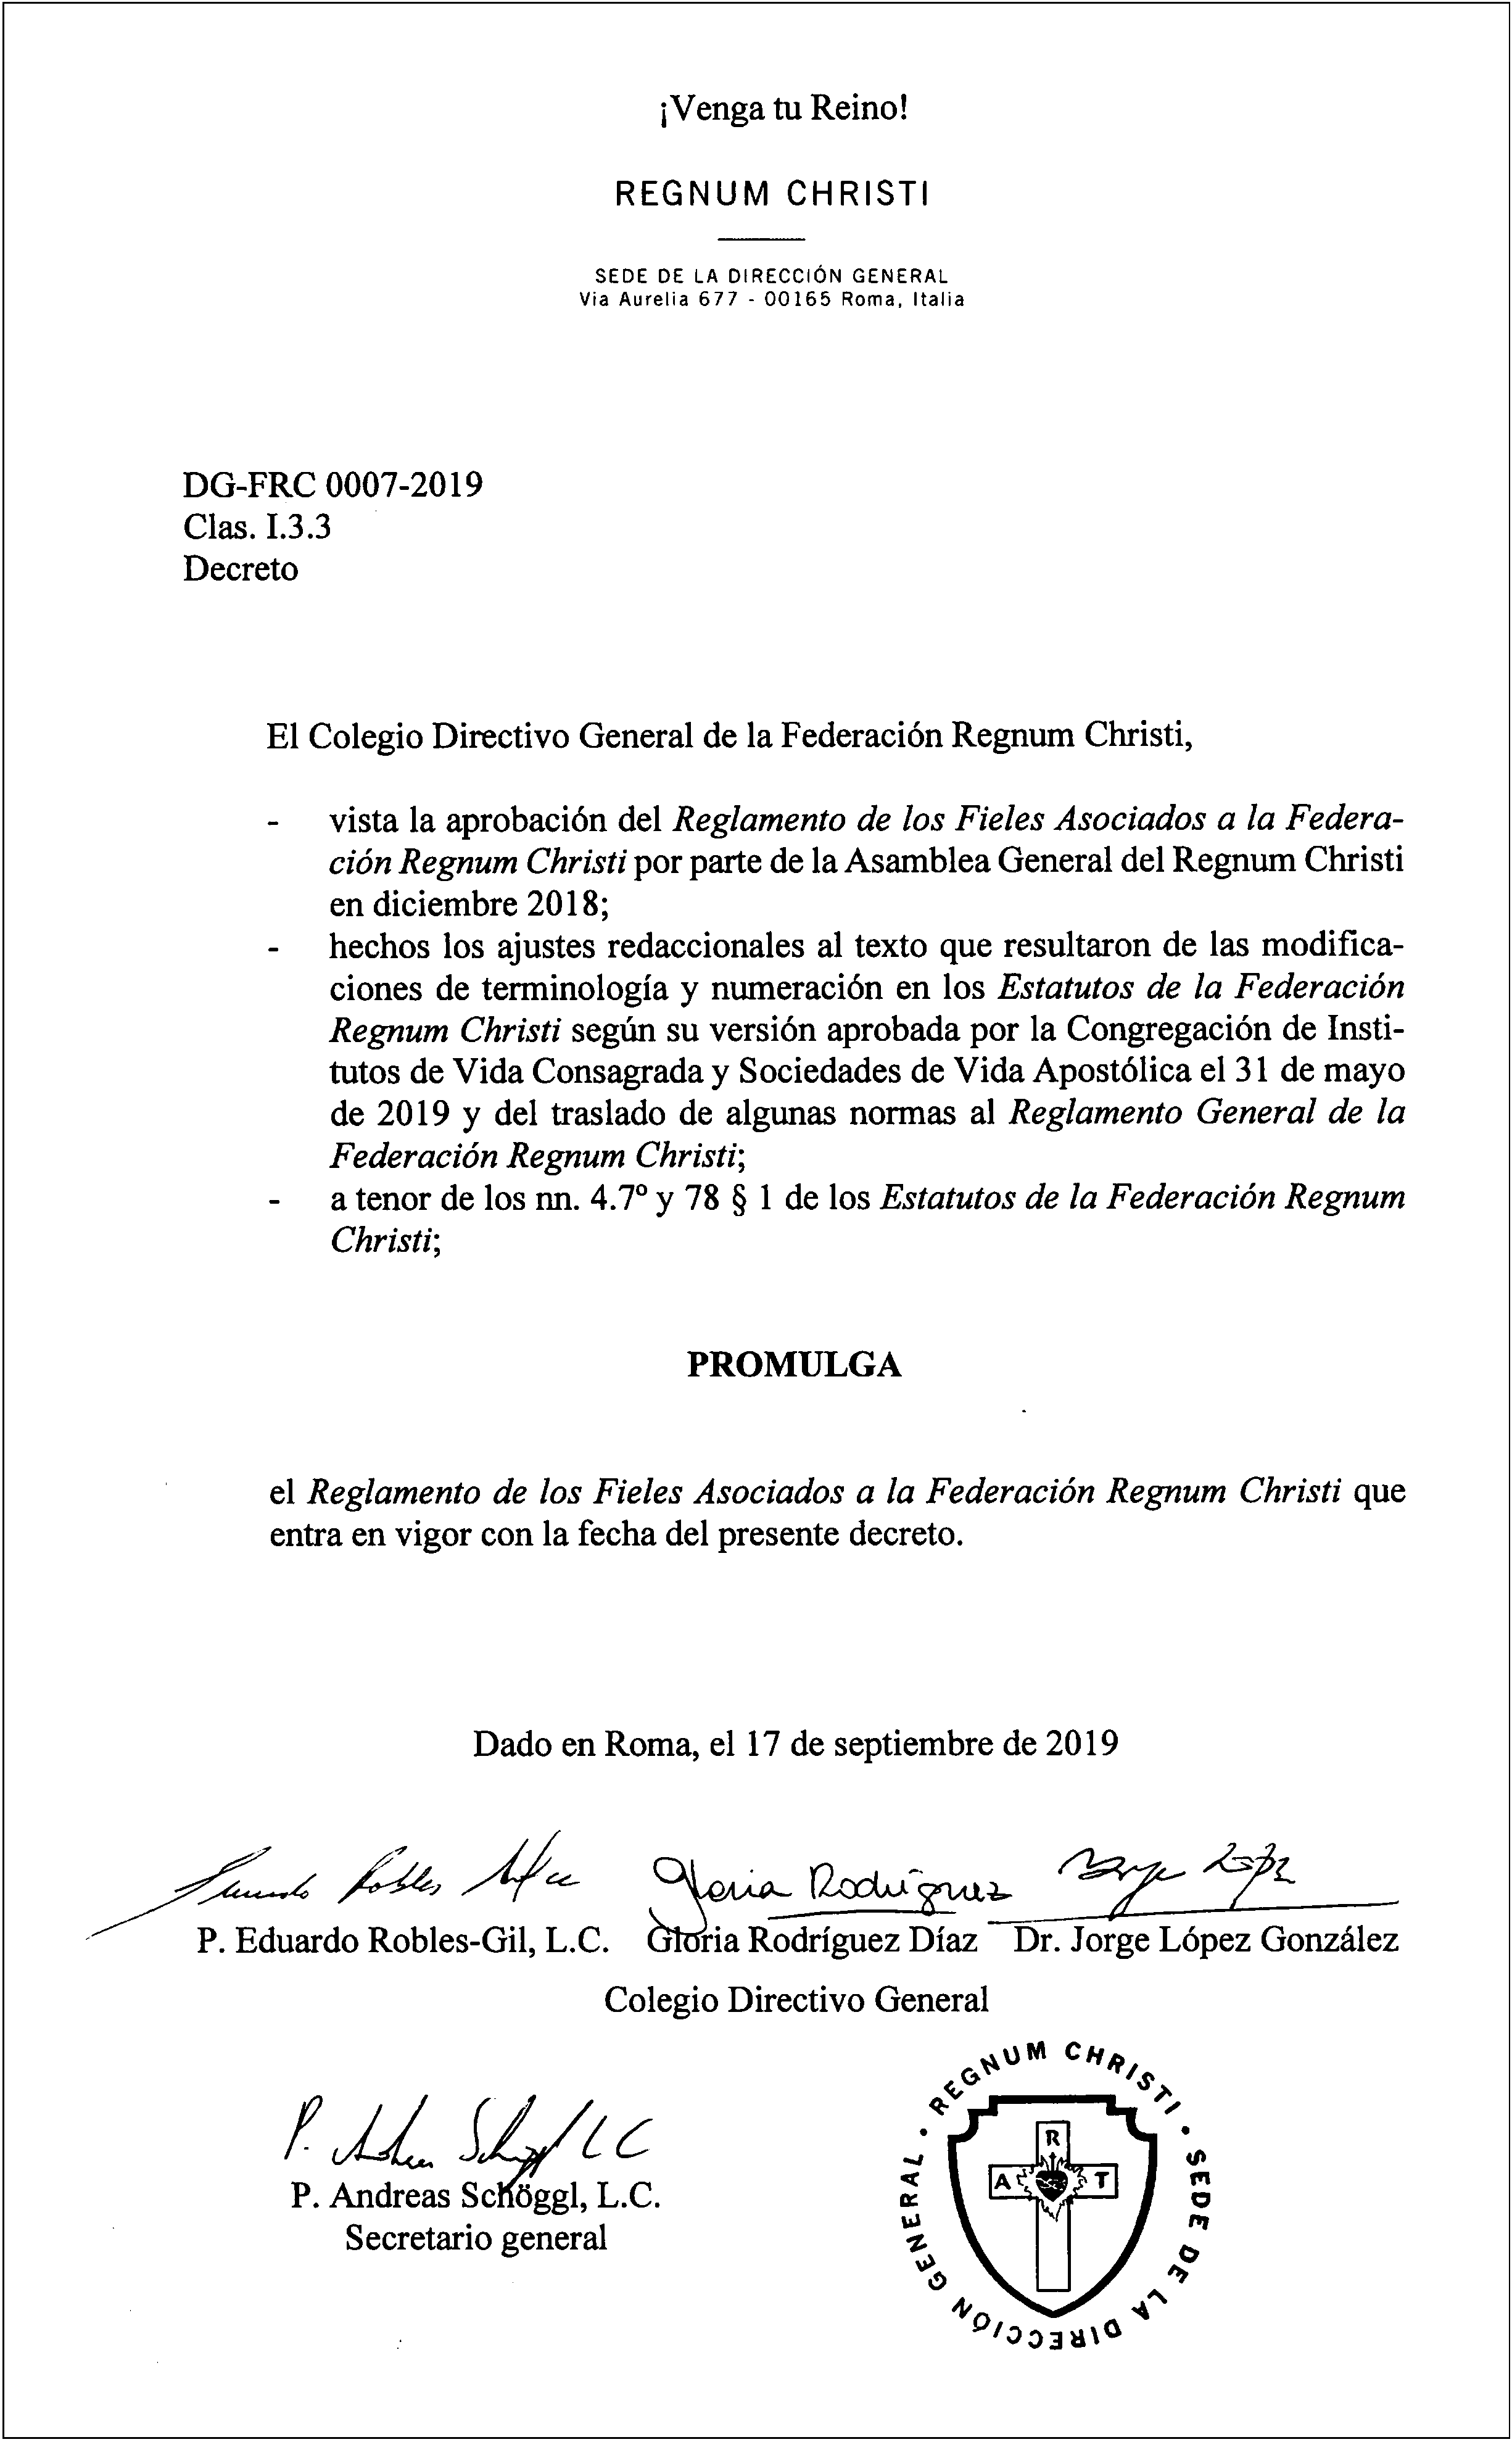
\includegraphics[height=\textheight]{dekret-przepisy-wiernych-stowarzyszonych}
\end{center}


\begin{framed}
\begin{footnotesize}
\begin{center}
Przyjdź Królestwo Twoje!


REGNUM CHRISTI\\
Siedziba Zarządu Generalnego\\
Via Aurelia 677, 00165 Rzym, Włochy
\end{center}
 
DG – FRC007-2019\\
Clas. I.3.3\\
Dekret
 
Kolegium Generalne Federacji Regnum Christi,


\begin{itemize}


\item zatwierdziwszy w grudniu 2018 roku, decyzją Zgromadzenia Ogólnego Regnum Christi, Przepisy Wiernych Stowarzyszonych w Federacji Regnum Christi;


\item uwzględniwszy dostosowania w redakcji tekstu wynikające ze zmian terminologii i numeracji Statutów Federacji Regnum Christi według wersji zatwierdzonej 31 maja 2019 roku przez Kongregację ds. Instytutów Życia Konsekrowanego i Stowarzyszeń Życia Apostolskiego, wynikających również z przeniesienia niektórych norm do Przepisów Ogólnych Federacji Regnum Christi;


\item zgodnie z wytycznymi punktów 4.7. i 78 \S{}1 {\em Statutów Federacji Regnum Christi};


\end{itemize}


\begin{center} 
PRZYJMUJE
\end{center}
 
{\em Przepisy Wiernych Stowarzyszonych w Federacji Regnum Christi}, które wchodzą w życie wraz z datą wystawienia niniejszego dekretu.
 
\begin{center}
Podpisano w Rzymie, 17 września 2019 roku


\begin{tabular}{ c c c }
{\em podpis} & {\em podpis} & {\em podpis} \\
o. Eduardo Robles-Gil, LC & Gloria Rodríguez Díaz & dr. Jorge López González \\
\multicolumn{3}{c}{Kolegium Generalne} 
\end{tabular}


\begin{tabular}{ c c c }
{\em podpis} & & \\
o. Andreas Schöggl , LC & & {\em pieczęć} \\
Sekretarz Generalny & & 
\end{tabular}


\end{center}


\end{footnotesize}
\end{framed}
 
% Część pierwsza
\part{Świeccy członkowie Federacji}


%Rozdział 1
\chapter{Tożsamość i styl życia świeckiego członka Regnum Christi}
 
\ssec{Tożsamość świeckiego członka Regnum Christi}
 
\lett{1} \S{}1. „Świeccy członkowie Regnum Christi” to wierni, którzy bez przyjmowania zobowiązań ewangelicznych w relacji duchownej osobiście odpowiadają na Boże powołanie do przeżywania zobowiązań chrzcielnych w rzeczywistości doczesnej i według charyzmatu  Regnum Christi, którego fundamentalne założenia zostały opisane w punktach  6-30 {\em Statutów Federacji Regnum Christi} oraz w niniejszych {\em Przepisach}.


\S{}2. Wierni ci przystępują do Regnum Christi poprzez osobiste członkostwo w Federacji i zatwierdzani są przez dyrektorów jej poszczególnych sekcji.


\S{}3. Wnoszą oni swoje świeckie usposobienie i apostolską działalność, które uobecniają Chrystusa w świecie i poszukują drogi do ewangelicznej przemiany ludzkiej rzeczywistości, zwłaszcza w aspekcie życia rodzinnego, zawodowego i społecznego.\footnote{{\em Statuty Federacji Regnum Christi}, 5 \S{}4.}
 
\ssec{Elementy właściwe dla stylu życia świeckiego członka Regnum Christi}
 
\lett{2} Regnum Christi proponuje chrześcijaństwo aktywne i radosne w miłości, proponuje taki styl życia, który pomaga żyć według zobowiązań chrzcielnych i realizować misję bycia chrześcijańską solą dla ziemi. Świecki członek Regnum Christi rozwija jego styl życia w życiu duchowym, w formacji, apostolacie, osobistym uczestnictwie i w życiu we wspólnocie.


\section{Artykuł 1. Życie duchowe}


\ssec{Ukierunkowanie życia duchowego}


\lett{3} Świecki członek Regnum Christi postrzega życie duchowe jako ciągły rozwój życia trynitarnego w sobie samym, prowadzący do upodabniania się do Chrystusa. Z tej przyczyny przeżywa on swoje życie jako dynamiczną relację miłości z Bogiem, życie które odżywia się sakramentami, Słowem Bożym, życiem liturgicznym, modlitwą oraz doskonaleniem cnót teologicznych i moralnych. Życie duchowe przenika i harmonizuje wszystkie obszary życia.


\ssec{Świecka duchowość}


\lett{4}{} Świadomy otrzymanego na Chrzcie św. daru przynależności Bożej w Chrystusie, świecki członek Regnum Christi wypełnia swoją kapłańską, proroczą i królewską posługę w doczesnej rzeczywistości, dążąc do uobecniania Królestwa Boga na tym świecie tak, by stał się on domem godnym synów Boga, w którym wszystko sprowadza się do oddawania Mu chwały.
 
\ssec{Praktyka życia duchowego}
 
\lett{5} Praktyki życia duchowego proponowane świeckim członkom Regnum Christi są sposobem wzrastania w relacji miłości z Chrystusem. Świecki członek, dzięki pomocy swojego duchowego kierownika, stopniowo zagłębia się w mentalną modlitwę oraz w przeżywanie innych, zalecanych w Modlitewniku praktyk. Uprzywilejowanym sposobem osiągania wzrostu duchowego jest zalecane, coroczne uczestnictwo w ćwiczeniach duchowych albo w triduum odnowy wewnętrznej.


\section{Artykuł 2. Formacja}


\lett{6} Świecki członek Regnum Christi podejmuje ścieżkę formacji zgodnie z punktem 30. {\em Statutów Federacji Regnum Christi}. Ścieżka ta pomaga mu wzrastać w jego dojrzałości ludzkiej i chrześcijańskiej w odniesieniu do własnego życia, pomaga w skutecznej współpracy w apostolstwie oraz pomaga oświetlać i przemieniać różne oblicza świata w Chrystusie.
 
\ssec{Osobista odpowiedzialność i ścieżka instytucjonalna}


\lett{7} \S{}1. Świecki członek deklaruje osobistą odpowiedzialność za swoją własną formację.


\S{}2. Odpowiedni podmiot Federacji zobowiązany jest do wytyczenia mu takiej ścieżki formacyjnej, która podpowie jakie są cele, wskazówki i środki.


\S{}3. Standardowy sposób prowadzenia formacji oparty jest na kręgach studyjnych i zróżnicowanych kursach.
 
\ssec{Przygotowanie}


\lett{8} Świeccy członkowie Regnum Christi, którzy są wyznaczeni do wypełniania obowiązków dotyczących posługi innym muszą otrzymać odpowiednie przygotowanie, wsparcie oraz informację zwrotną.


\section{Artykuł 3. Apostolat}


\ssec{Bycie apostołem}


\lett{9} Świeccy członkowie Regnum Christi gorliwie poszukują ustanowienia i rozpowszechnienia Królestwa Chrystusa wśród ludzi. Pozwalają, by przenikała ich troska Chrystusa w stosunku do ludzkości oraz ożywiają swój zapał apostolski w bliskim kontakcie z Chrystusem. Pragną, by Chrystus zawładnął ich własną duszą i duszą wszystkich tych, którzy ich otaczają. Kierowani Duchem Świętym i duchowością św. Pawła dążą do bycia wyjątkowymi w swoich aspiracjach, do bycia szczodrego serca, bycia śmiałymi w powierzeniu się, wytrwałymi wobec przeciwności losu oraz praktycznymi i skutecznymi w działaniu, poszukując tym samym przemiany świata w Chrystusie. Ich hasłem jest: {\em Chryste, Królu Nasz: Przyjdź Królestwo Twoje!} Wobec tego świeccy członkowie:


\begin{enumerate}


%1
\item szukają codziennego spotkania z Chrystusem w modlitwie oraz dają o Nim świadectwo w różnych okolicznościach swojego życia;


%2
\item w przeżywaniu swojego świeckiego powołania, oświeceni Słowem Bożym i nauczaniem Kościoła, w pierwszej kolejności biorą odpowiedzialność za swoje życie rodzinne i swoje obowiązki zawodowe;


%3
\item poszukują sposobów wyjścia na spotkanie z ludźmi w konkretnej sytuacji życiowej, aby móc głosić im Ewangelię i zapraszać ich do współuczestnictwa w misji Chrystusa;


%4
\item przyjmują świecką odpowiedzialność dostarczania światła Ewangelii w obręb życia publicznego, kulturalnego, gospodarczego, politycznego, akademickiego i społecznego; ponadto szukają sposobu na rozbudzenie apostolskiej powinności wśród przeróżnych liderów dzisiejszego świata, aby żyli oni w większej spójności ze swoimi etycznymi i religijnymi przekonaniami;


%5
\item w miarę możliwości podejmują inicjatywy i uczestniczą w dziełach apostolskich;


%6
\item szukają sposobów uczestniczenia w życiu parafialnym i diecezjalnym, wnosząc do swojego lokalnego Kościoła charyzmat Regnum Christi;


%7
\item pragną dzielić z innymi dar Boży odkryty dzięki Regnum Christi, dlatego umożliwiają jego poznanie, zapraszają do Regnum Christi i towarzyszą osobom, które okazują nim zainteresowanie lub chcą uczestniczyć w jego duchowości i misji.


\end{enumerate}
 
\ssec{Wartość ECYD (Spotkania, przekonania i decyzje)}


\lett{10} Pamiętając o tym, że młodzież to fundament przyszłości Kościoła, Regnum Christi oraz całego społeczeństwa, świeccy członkowie Regnum Christi są współodpowiedzialni za otaczanie odpowiednią troską i zainteresowaniem wszystkich młodych tworzących ECYD[WU2].


\section{Artykuł 4. Wsparcie osobiste i wspólnotowe}


\ssec{Wzajemne wsparcie[WU3]}


\lett{11} Wzajemne wsparcie\footnote{{\em Statuty Federacji Regnum Christi}, 35 \S{}1.} to wspólna odpowiedzialność świeckiego członka RC, który wsparcia poszukuje oraz Federacji Regnum Christi, która mu to wsparcie próbuje zapewnić. Urzeczywistnia się ono przede wszystkim w poszanowaniu osób i sakramentów, w życiu w zespole i formacji oraz w opiece apostolskiej.


\ssec{Przywództwo duchowe}


\lett{12} Świecki członek Regnum Christi poszukuje systematycznego przywództwa duchowego jako tradycyjnego w Kościele sposobu ku wzroście duchowemu. Dzięki niemu uczy się rozpoznawania woli Boga i przyjmowania jej z miłością.    


\ssec{Dialog z przełożonym}


\lett{13} Świecki członek Regnum Christi jest wspierany przez swojego przełożonego, czyli osobę odpowiedzialną za zespół, która poprzez częsty dialog, jak prawdziwy brat i przyjaciel pomaga mu na drodze wzrastania personalnego i apostolskiego.


\section{Artykuł 5. Życie w zespole}


\ssec{Zespół}


\lett{14} \S{}1. Świeccy członkowie zazwyczaj wchodzą w skład jednego zespołu. Zespół to naturalny obszar, gdzie wzrasta i rozwija się ich życie w Regnum Christi.


\S{}2. Zespół to ogół członków połączonych chrześcijańską więzią braterstwa, stworzony do wzajemnej pomocy na ich drodze uświęcania, formacji i pracy apostolskiej, powstały na wzór pierwszych wspólnot chrześcijańskich.


\S{}3. Zespoły, zupełnie jak wspólnoty apostołów, mogą być tworzone na różne sposoby, w zależności od konkretnych możliwości regionu Federacji.
 
\ssec{Spotkanie z Chrystusem}


\lett{15} Spotkanie z Chrystusem jest istotą życia zespołu. W jego trakcie świeccy członkowie, jako wspólnota wiary prowadzona światłem Słowa Bożego, dokonują analizy swojego życia chrześcijańskiego; rozpoznają czego oczekuje od nich Pan, aby móc ewangelizować rzeczywistość, w której żyją; ożywiają się we własnym podążaniu za Chrystusem oraz hartują swój zapał apostolski.


% Rozdział 2
\chapter{Stowarzyszenie świeckich członków Regnum Christi}


\ssec{ Duchowe znaczenie aktu przyłączenia do Federacji}


\lett{16} Świecki członek stowarzyszony w Federacji świadomie podejmuje się chrzcielnego zobowiązania do świętości i apostolatu oraz powierza się Chrystusowi, aby to On królował w jego sercu i w społeczności. W ten sposób rozpoczyna swą drogę upodabniania do Chrystusa i życie według ducha, wspólnoty i misji Regnum Christi opisanych w {\em Statutach Federacji Regnum Christi}, a szczególnie w pięciu niezbędnych  elementach życia świeckiego członka Regnum Christi\footnote{{\em Statuty Federacji Regnum Christi}, 2.}.
 
\ssec{Zobowiązania}


\lett{17} Świecki członek w momencie zrzeszenia się w Federacji zobowiązuje się do  przestrzegania następujących wytycznych:


\begin{enumerate}


%1
\item wzrastania w przyjaźni z Chrystusem rozwijając życie w łasce poprzez modlitwę i sakramenty;


%2
\item przeżywania ewangelicznych cnót ubóstwa, synowskiego posłuszeństwa oraz czystości myśli i czynów;


%3
\item wypełniania z miłością i uczciwością obowiązków wynikających z powierzenia swojego życia posłudze Bogu i innym ludziom;


%4
\item wytrwałej formacji ogólnej i kształtowania swego chrześcijańskiego przywództwa;


%5
\item podejmowania inicjatyw apostolskich i uczestnictwa w nich;


%6
\item wyznawania wiernej i aktywnej miłości do świętego Kościoła, Ojca Świętego i poszczególnych biskupów;


%7
\item hojnego ofiarowania swej modlitwy, talentów, czasu i pracy na rzecz współtworzenia misji Regnum Christi ku posłudze Kościołowi.


\end{enumerate}


\ssec{Wymagania}


\lett{18} Do stowarzyszenia może wstąpić każdy katolik, który ukończył szesnasty rok życia, pragnie żyć duchem Regnum Christi, posługiwać się jego środkami uświęcania i współuczestniczyć w jego apostolskiej posłudze, a ponadto wykazuje się prawym postępowaniem oraz potrafi podjąć się wypełniania nowych obowiązków.


\ssec{Przynależność do innych ruchów kościelnych}


\lett{19} \S{}1. Ci, którzy przynależą już do innych ruchów kościelnych, a pragną być zrzeszeni w Federacji powinni wraz z dyrektorem sekcji rozważyć, czy ich zobowiązania zgadzają się z tymi wcześniejszymi, podjętymi w innych instytucjach.


\S{}2. Nie wyraża się zgody na dołączenie do Federacji osobom, które uprzednio podjęły rady ewangeliczne potwierdzone świętym węzłem w innej rodzinie duchowej.


\ssec{Proces przyłączenia}


\lett{20} \S{}1. Decyzja o chęci przyłączenia do Federacji musi być owocem odpowiedniego rozeznania i swobodnej odpowiedzi na wezwanie Boga.


\S{}2. Przyjęcie do Federacji leży w kompetencji dyrektora sekcji, odbywa się na pisemny wniosek ubiegającej się o przyjęcie osoby oraz na mocy rekomendacji wydanej przez osobę odpowiedzialną  za zespół, a także jednego z członków tego zespołu i następuje po odpowiednim okresie uczestnictwa w życiu Regnum Christi, które służyło wzajemnemu poznaniu się osoby zainteresowanej i dyrektora sekcji.


\S{}3. Przyjęcie do stowarzyszenia zazwyczaj odbywa się po triduum duchowym, poprzez formalny akt lub ceremonię, według założeń {\em Ceremoniału Regnum Christi}, o czym również wspomina 16. i 17. punkt niniejszych {\em Przepisów}. Przyjęcie do stowarzyszenia zostaje odpowiednio odnotowane w aktach.


\S{}4. Świecki członek dokonuje corocznego modlitewnego odnowienia przyjętych z tytułu zrzeszenia zobowiązań, które ustanawia punkt 17. niniejszych {\em Przepisów}.


\S{}5. Członkowie stowarzyszonych instytucji, którzy opuszczają swoją instytucję i pragną nadal przynależeć do Regnum Christi powinni wnioskować u dyrektora sekcji o wpisanie ich w rejestr świeckich członków Regnum Christi.
 
\ssec{Odejście}


\lett{21} \S{}1. Każdy świecki członek Regnum Christi, po uprzednim rozważeniu przed Bogiem swojego odejścia, ma prawo do opuszczenia Federacji po pisemnym zawiadomieniu swojego dyrektora sekcji.


\S{}2. Zgodnie z całkowicie dobrowolnym i bezinteresownym osobistym zobowiązaniem, osoba opuszczająca Federację, niezależnie od sposobu swojego odejścia, nie ma prawa żądać niczego z tytułu jakiegokolwiek rodzaju świadczeń na rzecz Federacji.


\ssec{Utrata przynależności ipso facto[WU4] }


\lett{22} \S{}1. Ipso facto przestają przynależeć do Federacji Regnum Christi osoby, które podejmują rady ewangeliczne potwierdzone świętym węzłem w innej rodzinie duchowej.


\S{}2. Również ten, kto publicznie porzuca wiarę katolicką ipso facto przestaje być już zrzeszonym w Federacji Regnum Christi.
 
\ssec{Wydalenie i jego powody}
 
\lett{23} \S{}1. Dyrektor sekcji po uprzednim wysłuchaniu odpowiedzialnego za zespół oraz za zgodą swojej Rady może, w oparciu o słuszne powody, wydalić świeckiego członka z Federacji, jeśli zajdzie taka potrzeba. Zanim zapadnie decyzja o jego wydaleniu, dyrektor sekcji, wysłuchawszy odpowiedzialnego za zespół lub grupę oraz za zgodą swojej Rady, zobowiązany jest do pisemnego upomnienia członka, w którym to musi przestrzec go o możliwości wydalenia z Federacji z podaniem konkretnego powodu. Upomnienie musi określić termin na ewentualną poprawę ze strony członka Federacji. Ma on prawo do obrony przed dyrektorem sekcji. Po upłynięciu wyznaczonego w upomnieniu terminu oraz po skorzystaniu przez wydalanego członka z możliwości obrony, dyrektor sekcji, jeśli uzna jego wydalenie za konieczne, zgodnie z decyzją swojej Rady, zobowiązany jest do pisemnego powiadomienia członka Federacji o jego wydaleniu. Samo wydalenie z Federacji musi odbyć się w sposób sprawiedliwy, rozsądny i miłosierny.


\S{}2. Wydalonemu świeckiemu członkowi Regnum Christi przysługuje prawo złożenia odwołania się do Kolegium Generalnego.


\S{}3. Powodem wydalenia jest publiczne i wytrwałe głoszenie idei lub zwyczajów sprzecznych z wiarą i nauczaniem Kościoła.


%Rozdział 3
\chapter{Szczególne sposoby powierzenia się świeckich członków Regnum Christi}


\section{Artykuł 1. Obietnica powierzenia}
 
\lett{24} \S{}1. Niektórzy świeccy członkowie doświadczają pewnego wezwania Boga do przyjęcia wyjątkowej obietnicy oddania się Panu i gotowości względem Niego po to, by ożywiać życie i misję Regnum Christi. W odpowiedzi na to wezwanie podejmują się oni drogi modlitwy i formacji oferowanej przez Regnum Christi oraz zobowiązują się do aktywnego w niej uczestnictwa poprzez swoją modlitwę, talenty, czas i posługę.


\S{}2. Osoby przyjmujące to wezwanie udzielają wartościowego wsparcia sekcjom oraz swoim apostolatom poprzez modlitwę, oddanie i dyspozycyjność.


\S{}3. Świecki członek Regnum Christi oraz dyrektor sekcji ustalają między sobą różne konkretne formy przeżywania tego oddania i dyspozycyjności w zależności od osobistych okoliczności życia członka, jak również od potrzeb Regnum Christi.


\S{}4. To świecki członek Regnum Christi, wspierany przez swojego duchowego dyrektora[WU5] , bierze na siebie odpowiedzialność godzenia podejmowanych zobowiązań z własnymi obowiązkami życia codziennego.




\lett{25} \S{}1. Podjęcie tych wyjątkowych zobowiązań wobec Regnum Christi odbywa się poprzez obietnicę powierzenia złożoną w obecności dyrektora sekcji i kilku jej członków oraz według zasad Ceremoniału Regnum Christi.


\S{}2. Obietnica powierzenia wymaga pisemnej adnotacji w aktach.


\S{}3. Pierwsza obietnica powierzenia składana jest na okres jednego roku z możliwością corocznego przedłużenia. Po pięciokrotnym wznawianiu obietnica ulega przedłużeniu {\em ad vitam aeternam}, o ile taka jest wola świeckiego członka Regnum Christi i dyrektora sekcji.
 
\ssec{Przepis przejściowy}


Odnośnie do poprzedniego punktu, ci świeccy członkowie Regnum Christi, którzy są uważani za tzw. „członków drugiego stopnia”, byli nimi co najmniej przez ostatnie pięć lat i posiadają zgodę dyrektora sekcji, będą mogli złożyć obietnicę powierzenia {\em ad vitam aeternam} bez potrzeby spełnienia warunków punktu 25, \S{}3 niniejszych {\em Przepisów}.


\S{}4. Dyrektorzy sekcji dbają o to, by członkowie składający obietnicę powierzenia otrzymywali niezbędne wsparcie w wypełnianiu swej obietnicy.


\S{}5. Właściwy organ Federacji zobowiązuje się do nakreślenia członkom składającym obietnicę odpowiedniej ścieżki formacji wyznaczającej cele, wskazówki i metody.
 
\ssec{Wymagania do złożenia obietnicy}


\lett{26} \S{}1. Obietnicę powierzenia może złożyć świecki członek Federacji, który ukończył osiemnasty rok życia, postępuje w sposób prawy, stowarzyszony jest w Federacji wystarczająco długo, by dać się poznać swojemu dyrektorowi sesji oraz z pomocą swojego duchowego przywódcy przeszedł przez etap rozeznania.


\S{}2. Obietnicę należy złożyć w duchu przychylności i pokory wobec posługi Królestwu Bożemu oraz w mocnym pragnieniu przyczynienia się do rozwoju Regnum Christi.
 
\ssec{Przyjęcie}


\lett{27} Przyjęcie obietnicy leży w gestii dyrektora sekcji oraz jego Rady i odbywa się na pisemny wniosek osoby zainteresowanej.
 


\ssec{Dyspensa}


\lett{28} \S{}1. Świecki członek Regnum Christi po dojrzałym rozeznaniu dokonanym przy wsparciu swojego duchowego dyrektora[WU6]  może wnioskować u dyrektora sekcji o zwolnienie z obietnicy powierzenia.


\S{}2. Dyrektor sekcji udziela świeckiemu członkowi dyspensy w formie pisemnej, co też zostaje odnotowane w archiwum sekcji.


\section{Artykuł 2. Współpracownicy}
 
\ssec{Współpracownicy}


\lett{29} Mianem współpracowników określani są ci świeccy członkowie Regnum Christi, którzy poświęcają przynajmniej jeden rok swojego życia na pełnowymiarową i bezpłatną służbę apostolską Kościołowi poprzez Regnum Christi i według jego przepisów.


%Rozdział 4
\chapter{Struktura i funkcje życiowej posługi świeckich członków Regnum Christi}


\ssec{Zespoły}


\lett{30} \S{}1. Zespół składa się przeważnie z osób tej samej płci, będących na tym samym etapie życia, połączonych więzią przyjaźni, podobieństwa lub wspólnych zainteresowań. Istnieją również zespoły małżeństw prowadzone przez jedno małżeństwo.


\S{}2. Zespół prowadzony jest przez jedną osobę za niego odpowiedzialną, wyznaczoną przez dyrektora sekcji na okres od jednego do trzech lat z możliwością przedłużenia funkcji; wspieraną przez przydzieloną mu Radę i opinie pozostałych członków zespołu.


\S{}3. Misją osoby odpowiedzialnej za zespół jest prowadzenie i ożywianie życia w zespole. Jest on przewodnikiem i wychowawcą, który towarzyszy każdemu członkowi w jego drodze uświęcania, w procesie formacji i w jego rozwoju jako apostoła.


\S{}4. Liczba członków w zespole powinna sprzyjać wzajemnemu wsparciu, przyjaźni zawiązywanej między członkami oraz aktywnemu uczestnictwu każdego z nich.
 
\ssec{Grupy}


\lett{31} \S{}1. W stosownych przypadkach: z powodu formacji lub apostolatu, lub jeśli pozwala na to wystarczająca liczba zespołów, dyrektor sekcji może dokonać podziału zespołów na grupy.


\S{}2. Na czele każdej grupy stoi osoba za nią odpowiedzialna, wybrana przez dyrektora sekcji na okres do trzech lat z możliwością przedłużenia swej funkcji za przyzwoleniem osób odpowiedzialnych za zespoły.
 
\ssec{Sekcje}


\lett{32} \S{}1. Sekcja to zbiór zespołów i grup, które promują życie w modlitwie, kompleksową formację, rodzinnego ducha Regnum Christi, ideę zapraszania i przyjmowania nowych członków, wzajemne wsparcie, aktywność apostolską i zdrową gospodarność[WU7] .


\S{}2. Zazwyczaj istnieje sześć sekcji: męska, kobieca, męska sekcja młodych, damska sekcja młodych oraz sekcje ECYD, damska i męska.


\S{}3. Stworzenie lub usunięcie sekcji w danym regionie podlega decyzji Terytorialnego Kolegium Federacji na wniosek lokalnego dyrektora i służy wsparciu ogólnej misji, osobistej opiece i zapewnieniu organizacji wydajności.


\ssec{Dyrektor sekcji}
 
\lett{33} \S{}1. Terytorialne Kolegium Federacji po konsultacji z dyrektorem lokalnym, zgodnie z punktem 52 \S{}2 {\em Statutów Federacji Regnum Christi}, powołuje w każdej sekcji odpowiedniego dyrektora sekcji na okres trzech lat z możliwością przedłużenia funkcji. W sytuacjach wyjątkowych może być on również mianowany na okres jednego lub dwóch lat.


\S{}2.  Dyrektorem sekcji musi być świecki członek Regnum Christi stowarzyszony w Federacji co najmniej trzy lata albo członek zrzeszonej instytucji posiadający przynajmniej trzyletnie doświadczenie w pracy zespołowej.


\S{}3. Misja dyrektora sekcji polega na promowaniu celów sprecyzowanych w punkcie 32 \S{}1 niniejszych {\em Przepisów}.


\ssec{Organ Rady dyrektora sekcji}


\lett{34} \S{}1. Dyrektor sekcji posiada swój organ doradczy zwany Radą, która składa się przynajmniej z czterech świeckich członków Regnum Christi.


\S{}2. Członkowie Rady mianowani są przez dyrektora lokalnego na wniosek dyrektora sekcji. Ich funkcja trwa tyle, co funkcja dyrektora sekcji, z możliwością jej przedłużenia.


\S{}3. Dyrektor sekcji podpiera się Radą przy podejmowaniu decyzji,  prosi ją o przyzwolenie i opinię, zgodnie z założeniami niniejszych {\em Przepisów} oraz kodeksu uzupełniającego.
 
\ssec{Kapelan sekcji}


\lett{35} \S{}1. Sekcja zazwyczaj dysponuje jednym kapelanem, który mianowany jest przez Kolegium Terytorialne.


\S{}2. Kapelan sekcji, podporządkowany autorytetowi dyrektora sekcji, propaguje oraz  ożywia życie liturgiczne i sakramentalne, a także bierze udział w duchowej formacji świeckich członków Federacji.


\ssec{Formatorzy[WU8] }


\lett{36} \S{}1. Wychowawcy formacyjni to świeccy członkowie lub członkowie instytucji zrzeszonych, którzy biorą udział w kierowaniu sekcją i są odpowiedzialni za formację jej członków. Zajmują się oni głównie duchowym przewodnictwem, kaznodziejstwem, programem aktywności sprzyjających formacji członków, przewodzeniem zespołom i grupom oraz kierowaniem aktywności apostolskich.


\S{}2. W swojej codziennej pracy podlegają dyrektorowi sekcji. To on troszczy się, by wychowawcy otrzymali odpowiednie przygotowanie i wsparcie w wykonywaniu powierzonych zadań.


%Rozdział 5
\chapter{Udział świeckich członków Regnum Christi w organach Federacji}


\ssec{Współudział i współodpowiedzialność świeckich członków Regnum Christi}


\lett{37} Zważając na specyfikę powołania świeckich członków do życia pełnią charyzmatu, a co za tym idzie, do współuczestniczenia w życiu i w misji Regnum Christi, {\em Statuty Federacji Regnum Christi} stanowią, że świeccy członkowie muszą uczestniczyć w kierowaniu Federacją oraz w określaniu własnego sposobu przeżywania charyzmatu. Niniejsze {\em Przepisy} przedstawiają konkretną wizję ich uczestnictwa.
 
\section{Artykuł 1. Wybór i współuczestnictwo w Konwencji[WU9]  Generalnej i Terytorialnej}
 
\ssec{Przepis uzupełniający do punktu 68 {\em Statutów Federacji Regnum Christi}}
 
\lett{38} Delegaci świeckich członków Regnum Christi na Konwencję Generalną są wybierani przez i spośród delegatów świeckich członków Konwencji Terytorialnej. Liczba delegatów świeckich członków na Konwencję Generalną została określona w {\em Przepisach Konwencji Generalnej}.


\ssec{Przepis uzupełniający do punktu 59 {\em Statutów Federacji Regnum Christi}}


\lett{39} \S{}1. Aby wprowadzić w życie zalecenia punktu 59 \S{}2 {\em Statutów Federacji Regnum Christi}, delegaci świeckich członków Regnum Christi na Konwencji Generalnej tworzą Kolegium, które umożliwia przedstawienie ich poglądu na sprawę.


\S{}2. Delegaci świeckich członków wraz z członkami instytucji stowarzyszonych mają prawo do głosowania w kwestiach zatwierdzenia lub zmiany regulaminu Konwencji Generalnej\footnote{{\em Statuty Federacji Regnum Christi}, 59 \S{}3.}. Taką samą metodę stosuje się w przypadku zatwierdzenia lub zmiany innych ewentualnych aktów normatywnych ściśle traktujących o życiu świeckich członków Regnum Christi.


\ssec{Przepis uzupełniający do punktu 71 {\em Statutów Federacji Regnum Christi}}


\lett{40} Delegaci świeckich członków Regnum Christi na Konwencję Terytorialną wybierani są przez i spośród świeckich członków danego terytorium, zgodnie ze szczegółowymi przepisami przyjętymi przez Kolegium Konwencji Terytorialnej i po wcześniejszej konsultacji na Plenarium[WU10]  Terytorialnym.
 
\section{Artykuł 2. Wybór i współpraca świeckich w Kolegium Generalnym i Terytorialnym}


\ssec{Przepis uzupełniający do punktu 89 \S{}2 {\em Statutów Federacji Regnum Christi}}


\lett{41} \S{}1. W Plenarium Generalnym bierze udział sześciu świeckich członków wybranych przez i spośród delegatów świeckich członków na Konwencji Generalnej.


\S{}1. W przypadku rezygnacji jednego z członków, Kolegium Generalne, po wysłuchaniu pozostałych świeckich członków wspierających Plenarium Generalne, mianuje jego zastępcę.
 
\ssec{Przepis przejściowy}


Wybór świeckich członków w Kolegium Generalnym oraz tych obecnych na Plenarium Generalnym w okresie pomiędzy zatwierdzeniem {\em Statutów Federacji Regnum Christi} przez Stolicę Apostolską a zwołaniem najbliższej Konwencji [WU11] Generalnej, należy do kompetencji Kolegium Generalnego.
 
\ssec{Przepis uzupełniający do punktu 76 \S{}3 {\em Statutów Federacji Regnum Christi}}


\lett{42} Dwaj świeccy członkowie Kolegium Generalnego są wybierani przez Kolegium Generalne spośród sześciu świeckich członków biorących udział w Plenarium Generalnym.


\ssec{Przepis uzupełniający do punktu 21 \S{}3 {\em Statutów Federacji Regnum Christi}}


\lett{43} Świeccy członkowie Kolegium Terytorialnego, po wcześniejszej pozytywnej ocenie dyrektorów lokalnych, mianowani są przez Kolegium Terytorialne na okres kadencji trzech lat z możliwością jednokrotnego przedłużenia.


\ssec{Przepis uzupełniający do punktu 33 \S{}2 {\em Przepisów ogólnych Federacji Regnum Christi}}


\lett{44} Poza świeckimi członkami Kolegium Terytorialnego, na Plenarium Terytorialne zwołuje się również jednego lub kilku świeckich członków mianowanych przez to Kolegium Terytorialne, oczywiście po uprzedniej pozytywnej ocenie dyrektorów lokalnych.


\ssec{Konflikt interesów}


\lett{45} W przypadku konfliktu interesów wynikającego z poruszanych kwestii, Świeccy członkowie Regnum Christi obecni w Kolegium Generalnym lub Terytorialnym oraz ci uczestniczący w jego plenariach muszą zaprzestać działania lub, w stosownych przypadkach, zostaną oni odsunięci od funkcji przez Kolegium.


\ssec{Wydatki członków Kolegium kierowniczego}


\lett{46} Federacja zobowiązuje się do pokrywania wydatków związanych z wykonywaniem  posługi przez członków Kolegium Generalnego i Terytorialnego.
 
% Część 2
\part{Księża, diakoni i seminarzyści diecezjalni}


\ssec{Tożsamość księży, diakonów i seminarzystów diecezjalnych Regnum Christi}


\lett{47} \S{}1. Osobistej odpowiedzi na wezwanie do przeżywania swego kapłańskiego powołania według charyzmatu Regnum Christi mogą udzielić księża, diakoni i seminarzyści diecezjalni. 


\S{}2. Kapłani, diakoni i seminarzyści diecezjalni Regnum Christi przyłączają się do Federacji indywidualnie, zgodnie z zapisami niniejszych {\em Przepisów}.


\S{}3. Uczestniczą oni w duchowości, korzystają z metod uświęcania oraz duchowych i apostolskich zasobów oferowanych przez Regnum Christi.


\newpage
\vspace*{6cm}
\begin{center}
Per Regnum Christi ad Gloriam Dei


Przez Królestwo Chrystusa do Chwały Boga
\end{center}


\appendix


\chapter{Notatki oryginalnego tłumacza}


\begin{itemize}


\item  [WU1]A może ECYD zamienić na słowo SPiD, które jest skrótem od polskich liter?


\item  [WU2]Czy to jest kurs, krąg, apostolat,  a może jeszcze coś innego? Na razie nie mogę się tego domyślić z kontekstu… Chciałabym się dowiedzieć co kryje się za skrótem.


\item  [WU3]lub: współtowarzyszenie, akompaniament


\item  [WU4]Proszę zdecydować czy należy tłumaczyć ten łaciński zwrot.


\item  [WU5]Bardzo dziwnie to brzmi. Może przewodnika?


\item  [WU6]Przewodnika, przywódcy, kierownika?


\item  [WU7]Nie wiem czy chodzi o gospodarność czy raczej o finanse zespołów RC.


\item  [WU8]Takie słowo pojawia się w glosariuszu. Proszę spojrzeć do słownika języka polskiego. Słowo nie istnieje w kontekście formacji. Może wychowawcy albo formujący?


\item  [WU9]Jak mam rozumieć ustalone w glosariuszu słowo „konwencja”? Porozumienie, zgromadzenie? Nie jestem pewna, czy słowo „konwencja” jest odpowiednie w języku polskim.


\item  [WU10]Czy Plenarium to spotkanie czy grupa osób?


\item  [WU11]Ciągle mam problem z przyjętym glosariuszu słowem „konwencja”. Muszę wiedzieć, co to dokładnie oznacza w Regnum Christi.


\end{itemize}


\end{document}